\chapter{Sets and Logic}
\label{chsets}

\section{Sets and Elements}

The basic ``data type'' of mathematics is the \defini{set}. A set is a
collection (really just a fancy word for a container that can hold things)
of objects, which are called the \defini{elements} of the set.
We typically use squiggly parentheses $\{\,\}$ (often called ``curly
braces'') to denote a set.
For example,
imagine we have three objects, the number 2, and two other objects we call
$a$ and $b$. Then
\[
\{2,a,b\}
\]
is the set containing exactly these three objects. To refer to it we can give it
a name, $S=\{2,a,b\}$.
We can now make statements about which objects are elements of this set. For
example $2$ is an element of the set, while $3$ is not. We write this in
symbols (with $\in$ reading as ``is element of'') in the form
\[
2\in S,\qquad 3\not\in S
\]
We might also say ``$2$ is in $S$'' or ``$S$ contains $2$'', meaning exactly
the same.

Sets are characterized by their membership with two sets being equal if and
only if they have the same elements.
\begin{note}
Mathematicians try to be very exact in the language used. The expression {\em if
and only if} means that the property (or what is defined) -- here {\em two
sets are equal} -- holds under the given condition -- here {\em they have the same
elements} -- but not if the condition is violated.

An analog would be to describe an animal as an elephant if (and only if) it
is large, has large floppy ears and a trunk in place of the nose.
\medskip

A single {\em if} instead shows that one condition implies another, but is
not the only reason:
\begin{quote}
{\em If it is snowing outside, I wear gloves.}
\end{quote}
(but I also might be wearing them when it is cold and rainy).
\end{note}
When we describe sets
by enumerating elements it does not matter in which order we write down the
elements, nor if we write them down multiple times\mynote{Of course,
sometimes one might want to be able to describe objects with multiplicities.
We will see how to describe this below \pointer{secmultiset}}.
Thus
\[
S=\{b,1,a\}=\{a,1,a,1,b,b,a\}
\]
as sets, but
\[
S\not=\{1,2,3\},\quad S\not=\{a,b\},\quad S\not=\{2,a,a\},\quad
S\not=\{1,2,a,b\}.
\]

\subsection{Describing Sets}

In many cases, describing a set by enumerating all its elements is
hard or impossible. Thus two other techniques that are used. The first of
these is continuation with
$\ldots$ to indicate a pattern to be continued. For example, we might write
\[
E=\{\ldots,-4,-2,0,2,4,6,8,10,\ldots\}
\]
to describe the set of even integers. Similarly
$R=\{5,6,\ldots,10\}$ would describe the integers from $5$ to $10$, that is
$R=\{5,6,7,8,9,10\}$. The drawback of this method is that it relies on the
reader making the correct assumptions about the rule used to extend the
listed numbers. It thus -- and this is the second method -- is often easier
and better to spell out this rule explicitly as a property the objects must
have. We thus can write:
\[
R=\{x\mid \mbox{$x$ is integer and $5\le x\le 10$}\},
\]
read as ``The set of $x$ such that $x$ is an integer and $5\le x\le 10$''.

This notation can be quite powerful. The general pattern is to first
give a variable that stands for the elements of the set, possibly indicating
an(other) set that these elements are taken from. Next comes a separator,
we use a vertical line $\mid$ (but other punctuation marks such as $;$ or
$:$ are used as well). One can read this separator as ``such as''.
Finally follows the rule or condition that the elements need to satisfy to
be elements of the set.

Thus, if we use $\Z$ to denote the set of all integers, we could have
described the above examples as
$E=\{x\in\Z\mid \mbox{$x$ even}\}$ (read as ``The set of those integers $x$,
such that $x$ is even'') and $R=\{x\in\Z\mid 5\le x\le 10\}$.

The reason for specifying a set from which elements are chosen is to avoid
any ambiguity what kinds of objects are in the set (do we allow rational
numbers between $5$ and $10$ in the set $R$?), and to make the specification
clear.

Formally, this specification is called a {\em predicate}, using language from
grammar, in which a predicate is a part of a sentence that gives information
about the subject. For example, in the following sentence:
\[
\underbrace{\mbox{The house}}_{\mbox{{\em subject}}}\
\underbrace{\mbox{is painted green.}}_{\mbox{{\em predicate}}}
\]
\begin{defn}
A \defini{predicate} (for a given set $Y$) is a sentence, involving a
variable $x$, such that if we substitute $x$ by a particular element $a\in
Y$, the sentence becomes a statement that is either (and unambiguously)
true or false.
\end{defn}

For example, {\em $x$ has brown fur}, would be a possible predicate for the
set $Y$ of all animals, this predicate would be true for a brown bear, but
false for a frog.

Note that
determining the truth value of a predicate for a particular element
might be hard, or even impossible at a given time. (Imagine for example the
property for a sequence of words to occur in at least one book in a huge
library.)
But there cannot be ambiguity about whether the property is true for a
particular $x$. Thus, for
the set of pictures, {\em $x$ is art} would not be a predicate, while
{\em $x$ is letter size} would be one.
\smallskip

Finally, there is a variant that describes elements from transforming
elements of another set. (Sometimes
it is easier to describe what to do with elements, than to
give a property.)
We thus can write
$E=\{2y\mid y\in\Z\}$, using the property that even integers are exactly the
multiples of $2$.
\smallskip

For a set $A$, we define the \defini{cardinality}, denoted by $\sz{A}$ or
$\# A$ as the number of elements in $A$.\mynote{This is a somewhat vague
definition. We will give a more formal definition below
in~\pointer{defcardinality}}.

\subsection{Some common sets}

With much of mathematics working with numbers, it will be convenient to give
special names for some sets of numbers:
\begin{description}
\item[$\Z$] The integers, $\Z=\{\ldots,-3,-2,-1,0,1,2,3,4,\ldots\}$
\item[$\Q$] The rational numbers, fractions of integers.
$\Q=\{\frac{a}{b}\mid a,b\in\Z, b\not=0\}$.
\item[$\N$] The natural numbers $1,2,3,\ldots$. Often it is ambiguous
between different authors whether $0$ should be part of this, thus we will
write $\N_0$ (or $\Z_{\ge 0}$) if we want to guarantee that $0$ is an
element, respectively $\N_{>0}$ (or $\Z_{>0}$) if we explicitly want to
exclude $0$.
\item[$\R$] The real numbers on the number line. These numbers can be
described by possibly infinite decimal expansions. The proper, formal
definition however is more complicated and it will take us quite
a while (at the end of Chapter~\ref{chseqs}) to describe their formal
definition.
\end{description}


\section{Subsets}
\label{secsubsets}

With the basic operation for sets being a test for membership, an obvious
property for two sets $A,B$ is that one set contains every element of the
other.

\begin{defn}
If $A,B$ are sets, we call $A$ a \defini{subset} of $B$ if every element of
$A$ is also an element of $B$. That is $x\in A$ implies that $x\in B$
(formally: $x\in A\Rightarrow x\in B$). We write $A\subset B$.
When talking about sets being subsets of others, this is also called
\defini{inclusion} of subsets.
\end{defn}
\begin{note}
Some authors distinguish between {\em subset, could be equal} (symbol
$\subseteq$) and {\em proper subset, not equal} ($\subset$). We do not do
this and will state explicitly ($\subsetneqq$) if a subset is
proper (that is, not equal).
\end{note}

To provide for examples in this section, let
\begin{eqnarray*}
C&=&\{x\in\Z\mid 0\le x\le9\}=\{0,1,2,3,4,5,6,7,8,9\}\\
D&=&\{0,2,4\}\\
E&=&\{x\in\Z\mid \mbox{$x$ is even}\}\\
F&=&\{0,1,2\}.\\
\end{eqnarray*}
Then (for example) $D\subset C$, $D\subset E$, $C\not\subset D$,
$C\not\subset E$.

Since membership test is the basic operation for sets, one often reduces
equality of sets to two subset test:
\begin{lemma}
%\method{test equality of sets}
\label{lemseteq}
Let $A,B$ two sets. Then $A=B$ if and only if $A\subset B$ and $B\subset A$.
\end{lemma}
\begin{proof}
First assume that $A=B$. We want to show that $A\subset B$. For this, let
$x\in A$. Then $x\in B=A$, so $A\subset B$. By swapping the role of $A$ and
$B$ we get $B\subset A$ as well.

Vice versa, assume that $A\subset B$ and $B\subset A$. Then $x\in A$ implies
$x\in B$ and $x\in B$ implies $x\in A$, that is both sets have the same
elements and thus are equal.
\end{proof}

\subsection{The Empty Set}

It is often useful (for example for constructing certain sets, or to handle
borderline cases) to refer to the \defini{empty set} $\emptyset=\{\}$, that
is the set which contains no element. It is a subset of every set.

\subsection{Sets of Sets and Subtleties}

Sets can contain anything and thus one set can be an element of another set.
Indeed, this will be used later to build more complicated structures from
sets.
For example, if we have
\[
A=\{1,5,\{2,3\}\}
\]
then $1\in A$ and $\{2,3\}\in A$. Or consider
\[
B=\left\{S\subset\{1,2,3\}\bigm\mid
\sz{S}=2\right\}=\left\{\{1,2\},\{1,3\},\{2,3\}\right\}.
\]
In such situations, the wrapping level is important:
Being in a subset contained in another set is not the same as being an
element, i.e. $2\not\in A$. Nor is element the same as subset, we have
$\{2,3\}\in A$ but $\{2,3\}\not\subset A$, and indeed (note the extra
parentheses $\{\{2,3\}\}\subset A$. And of course $A\not=\{1,2,3,5\}$.

\subsection{The Power Set, Hasse diagrams}
\label{secpowerset}

The \defini{power set} of a set $X$ is the set
\[
{\cal P}(X)=\{S\mid S\subset X\}
\]
whose elements are the subsets of $X$, including the empty set and $X$
itself. For example, if $X=\{1,2,3\}$, then
\[
{\cal P}(X)=\left\{\{\},\{1\},\{2\},\{3\},\{1,2\},\{1,3\},\{2,3\},X\right\}.
\]
For a finite set $X$ with $\sz{X}=n$, we can describe the elements of the
power set by the bit\mynote{A bit is a variable that can have only two
values, often denoted by $0$ and $1$, or by ``false'' and ``true''.}-lists of length $n$: Given a subset $S\subset X$, we
form a bit-list by setting the $i$-th bit to $1$ if and only if the $i$-th
element of $X$ is contained in $S$. (Indeed, such bit-lists are good way of
representing the subsets of a set on a computer.) Thus there are as many
subsets as there are bit-lists, namely $2^n$ subsets of a set of size $n$.
\medskip

A convenient way of depicting the subsets of a set is the \defini{Hasse
diagram}\mynote{Named after the German mathematician \textsc{Helmut Hasse}
(1898-1979), who made effective use of such diagrams, but did not invent
them.}: sets are represented by dots (maybe labeled with the set name or
the set itself). If a set $A$ is contained in another set $B$, we place the
dot for $B$ higher than the dot for $A$, and connect the two dots by a line,
indicating that the lower placed set is contained in the higher placed one.
Finally, we leave out (or delete) lines, that indicate a connection that is
already implied by connections to an intermediate set. That is, if $A\subset
B$ and $B\subset C$ (and thus also $A\subset C$), we draw lines $A-B$ and
$B-C$, but not $A-C$. Figure~\ref{fighasse3set} shows the Hasse diagram for
the $8$ subsets of $X=\{1,2,3\}$. The actual diagram is given by the solid
lines. The grey dashed lines indicate set inclusions that will not be drawn,
as they are implied already by connections with intermediate sets.

\begin{figure}[t]
\begin{center}
%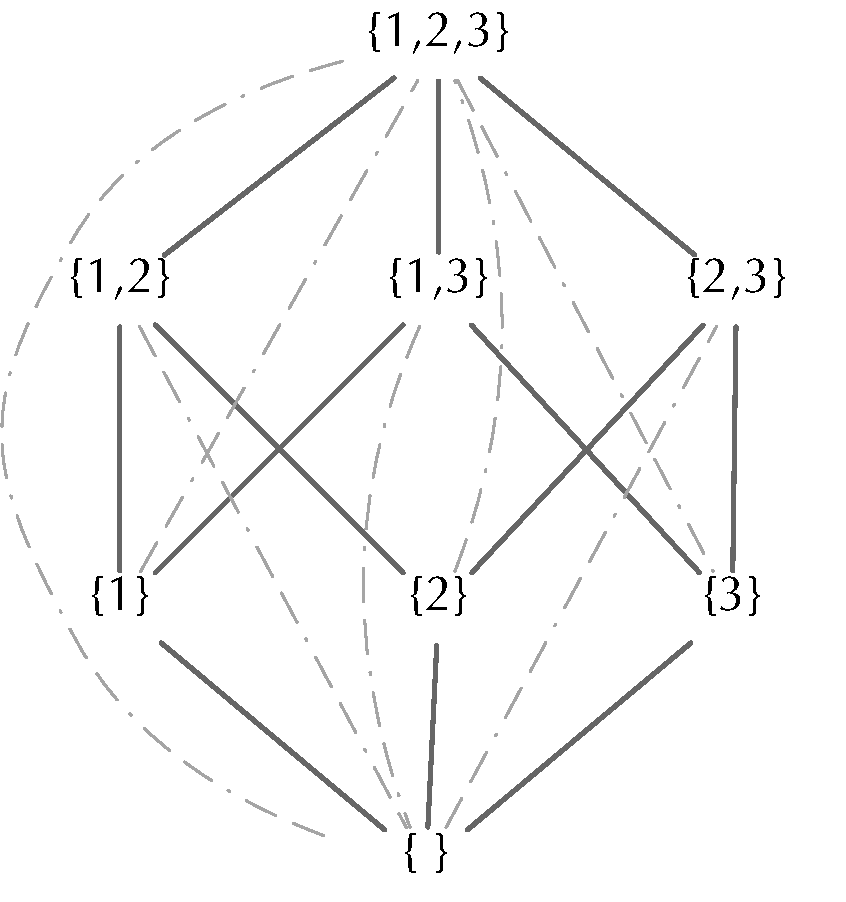
\includegraphics[width=4cm]{pic/Hasse3Set.pdf}
\anngraphics{4cm}{pic/Hasse3Set.png}{The Hasse diagram for all subsets of
the set {1, 2, 3} with lines connecting each subset to its parent set. The
complete arrangement resembles a cube shape.}
\end{center}
\caption{The Hasse diagram for all subsets of $\{1,2,3\}$.}
\label{fighasse3set}
\end{figure}

The same idea can be used, of course, for arbitrary sets and subsets.
Figure~\ref{fighasseV4} depicts the Hasse diagram for three different
collections of subsets of the $4$-element set $\{0,a,b,c\}$.

\begin{figure}[t]
\begin{center}
%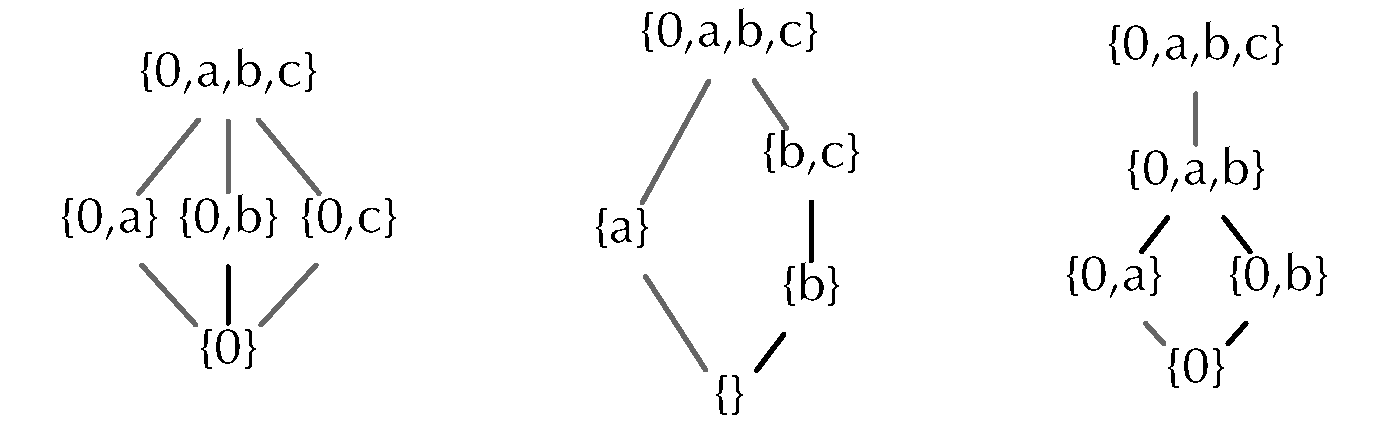
\includegraphics[width=8cm]{pic/HasseV4.pdf}
\anngraphics{8cm}{pic/HasseV4.png}{The Hasse diagram for all subsets of the
set {0, a, b, c} with lines connecting each subset to its parent set.
Various arrangements are given depending on subsets chosen.}
\end{center}
\caption{The Hasse diagram for certain subsets of $\{0,a,b,c\}$.}
\label{fighasseV4}
\end{figure}



\section{Intersection, Union, Difference, and Complement}

Next, we define a number of operations that construct new sets from old
ones, for example by taking common elements.
\begin{defn}
Let $A,B$ be two sets. The
\begin{description}
\item[\defini{intersection}] of $A$ and $B$ is the set of those elements
that are in $A$ and in $B$:
\[
A\cap B=\{x\in A\mid x\in B\}=\{x\in B\mid x\in A\}
\]
\item[\defini{union}] of $A$ and $B$ is the set of elements
that are in $A$, together with the elements in $B$:
\[
A\cup B=\{x\mid x\in A\quad\mbox{or}\quad x\in B\}
\]
\item[\defini{difference}] of $A$ and $B$ is the set of elements that are in
$A$ but not in $B$:
\[
A\setminus B=\{x\in A\mid x\not\in B\}.
\]
(Note that some authors simply write $A-B$.)

In the case that $B\subset A$ is understood from the context, this difference is sometimes called
the \defini{complement} of $B$ in $A$ and denoted by $B^\mycomplement$.
Clearly
\[
(B^\mycomplement)^\mycomplement=A\setminus(A\setminus B)=B
\]
\end{description}
\end{defn}
In the examples from Section~\ref{secsubsets}, we have that
$C\cap E=\{0,2,4,6,8\}$, $C\cap D=D$, $D\cap
F=\{0,2\}$, $D\cup F=\{0,1,2,4\}$, $C\cup D=C$, $C\setminus
D=\{1,3,5,6,7,8,9\}$, $D\setminus F=\{4\}$.
And if we assume that all sets are subsets of $C$ (such a set containing
everything in a given context is sometimes called an \defini{universe}), we
have that $D^\mycomplement=\{1,3,5,6,7,8,9\}$ and $C^\mycomplement=\emptyset$.

If they are included in a Hasse diagram (which does not hold for all
diagrams in Figure~\ref{fighasseV4}!), the union of two sets $A$ and $B$
will be the (minimal) dot above $A$ and $B$, the intersection the maximal
dot below $A$ and $B$.
\medskip

Another nice way of illustrating sets and the intersections and unions
is by using a \defini{Venn
diagram}, in which sets are represented by areas in the plane.
\figuref{figvennmulti} illustrates intersection, union and difference in
such a diagram, \figuref{figvenndiag} labels the 7 areas of a 3-set Venn
diagram.

\begin{figure}[t]
\begin{center}
%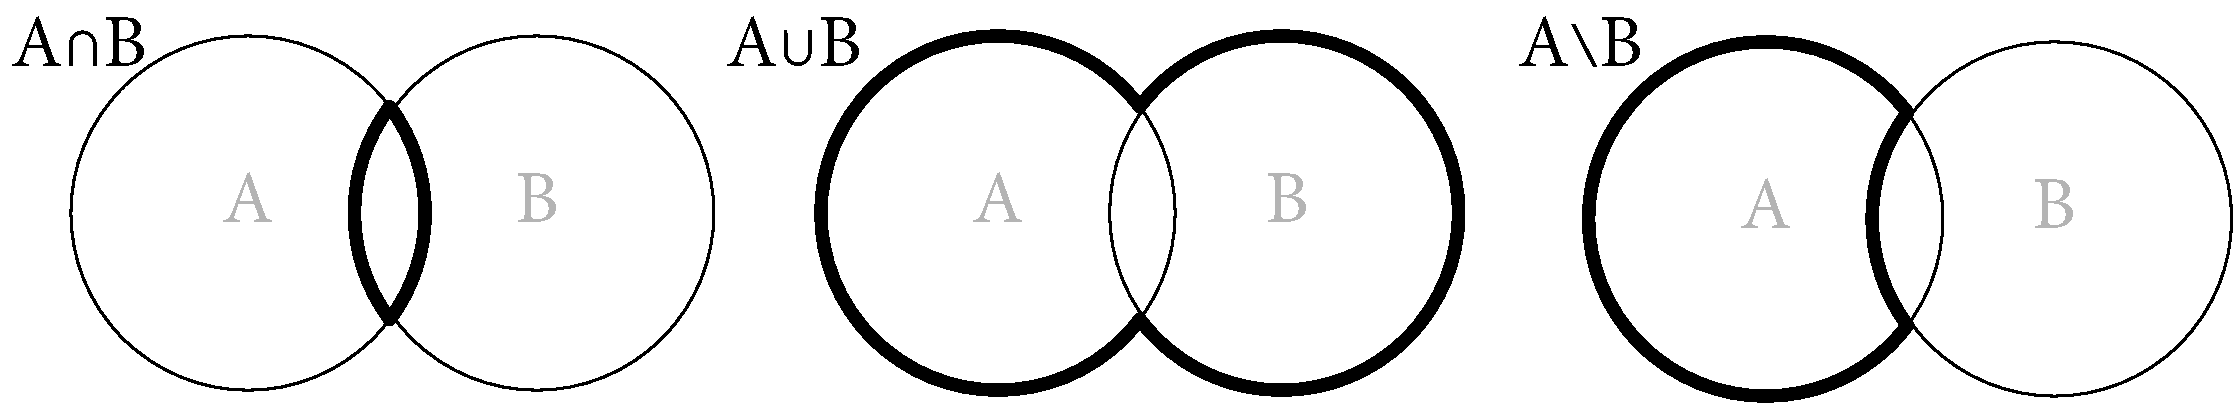
\includegraphics[width=10cm]{pic/VennMulti.pdf}
\anngraphics{10cm}{pic/VennMulti.png}{The concepts of intersection, union,
and difference are exemplified though the labelling of a Venn Diagram of two
circles representing sets A and B, respectively.}
\end{center}
\caption{Intersection, Union, and Difference}
\label{figvennmulti}
\end{figure}

\begin{figure}[t]
\begin{center}
%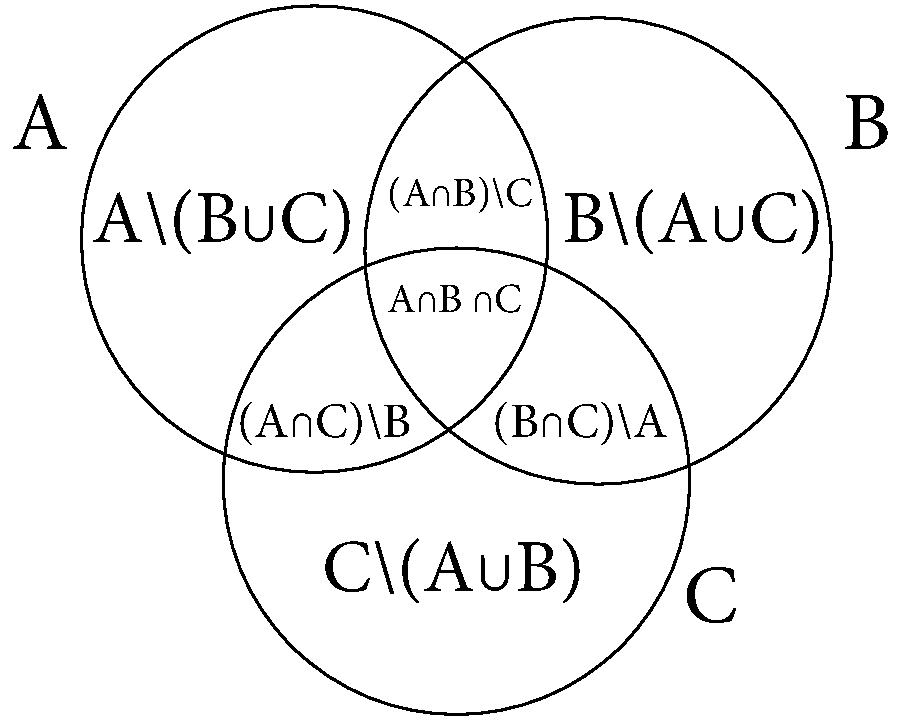
\includegraphics[width=6cm]{pic/VennDiagram.pdf}
\anngraphics{6cm}{pic/VennDiagram.png}{The concepts of intersection, union,
and difference are exemplified though the labelling of a Venn Diagram of
three circles which overlap, each of which represents a set A, B, or C
respectively.}
\end{center}
\caption{A Venn diagram for three sets}
\label{figvenndiag}
\end{figure}

We observe the following basic relations for these operations:
\begin{lemma}
Let $A,B,C$ be sets. Then
\begin{enumerate}
\item $A\cap B=B\cap A$.
\item $A\cup B=B\cup A$.
\item $A\cap B\subset A$.
\item $A\subset A\cup B$.
\item $A\setminus B\subset A$.
\item $(A\setminus B)\cup (A\cap B)=A$.
\item $(A\setminus B)\cap (A\cap B)=\emptyset$.
\item $(A\cap B)\cap C=A\cap (B\cap C)$ (so we can write $A\cap B\cap C$
without ambiguity).
\item $(A\cup B)\cup C=A\cup (B\cup C)$ (so we can write $A\cup B\cup C$
without ambiguity).
\end{enumerate}
\end{lemma}
Proofs are left as exercise for the reader.

\subsection{Distributive Laws}

The following properties are not trivial, but can be easily seen in a Venn
diagram:
\begin{thm}[Distributive laws]
Let $A,B,C$ be sets. Then (Figure~\ref{figvenndist}):\\
a) $A\cap (B\cup C)=(A\cap B)\cup(A\cap C)$.\\
b) $A\cup (B\cap C)=(A\cup B)\cap(A\cup C)$
\end{thm}
Note that these rules mimic what happens if we multiply by a sum: $a(b+c)$.
\begin{proof}
Since we have to show equality of sets, we need to show two-sided subset
inclusion.\\
a) We show first that $A\cap (B\cup C)\subset (A\cap B)\cup(A\cap C)$: For this,
let $x\in A\cap (B\cup C)$. This means that $x\in A$ and also $x\in B$ or
$x\in C$. In the first of these cases we have that $x\in A\cap B$, in the
second that $x\in A\cap C$. Thus in either case $x\in (A\cap B)\cup (A\cap
C)$. \\
For the reverse inclusion,
let $x\in (A\cap B)$. Then $x\in A$ and $x\in B\subset B\cup C$, so $x\in
A\cap (B\cup C)$. Similarly (swap $B$ and $C$) we see that $x\in A\cap C$
implies $x\in A\cap (B\cup C)$ as well. This show that
$A\cap (B\cup C)\supset (A\cap B)\cup(A\cap C)$.

b) Exercise
\end{proof}

\begin{figure}[t]
\begin{center}
%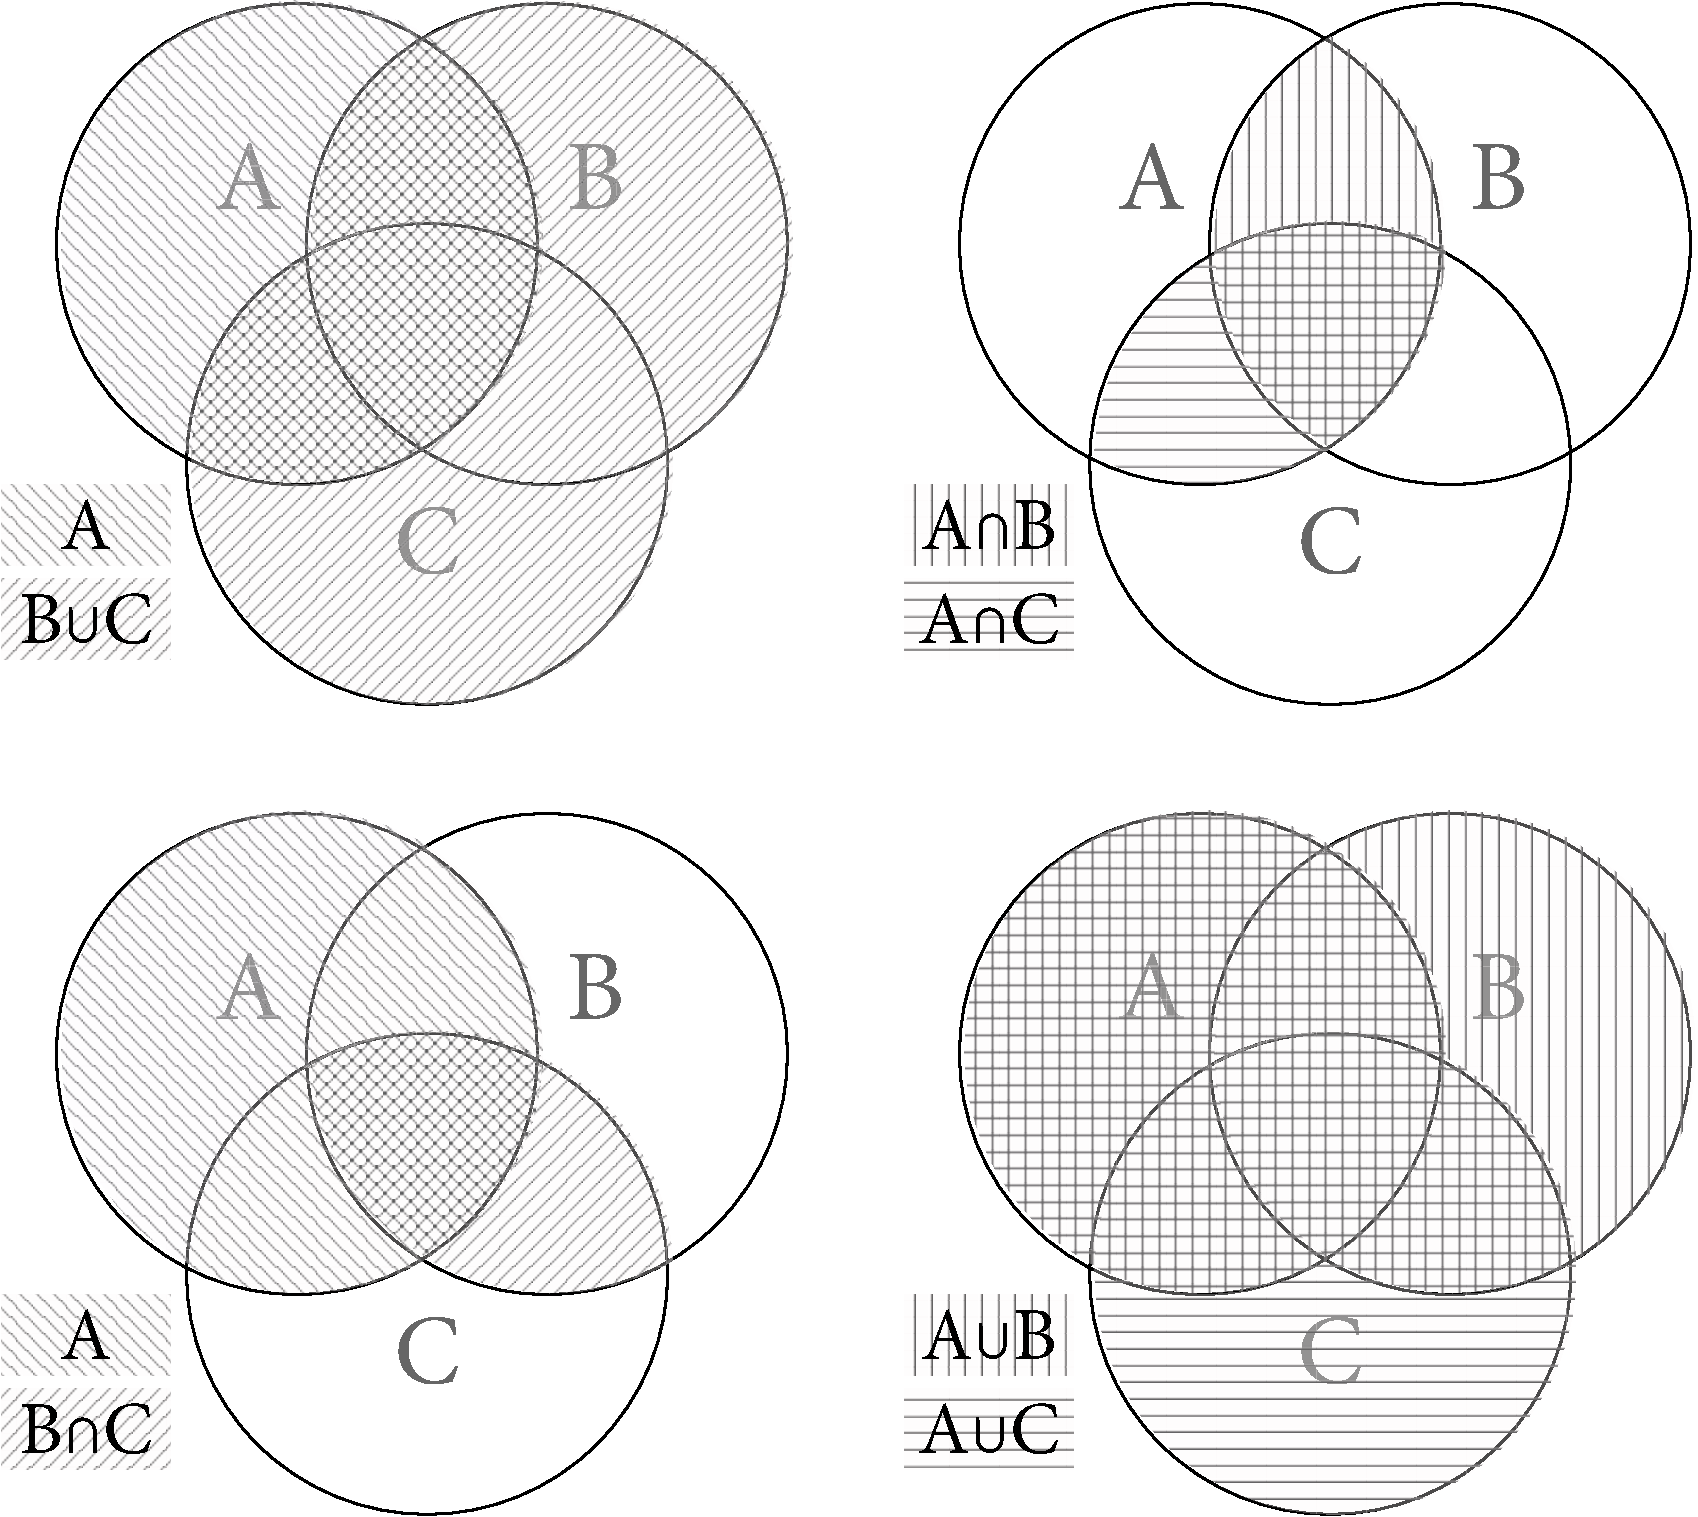
\includegraphics[width=6cm]{pic/VennDistributiveLaws.pdf}
\anngraphics{6cm}{pic/VennDistributiveLaws.png}{The Distributive Laws for
Union and Intersection are exemplified through the labelling and shading of
a Venn Diagram consisting of three circles which overlap, each of which
represents a set A, B, or C respectively.}
\end{center}
\caption{Distributive Laws for Union and Intersection}
\label{figvenndist}
\end{figure}

\subsection{De~Morgan's Laws}
\label{demorganlaws}

Next we look at rules to simplify complement operations

\begin{figure}[t]
\begin{center}
%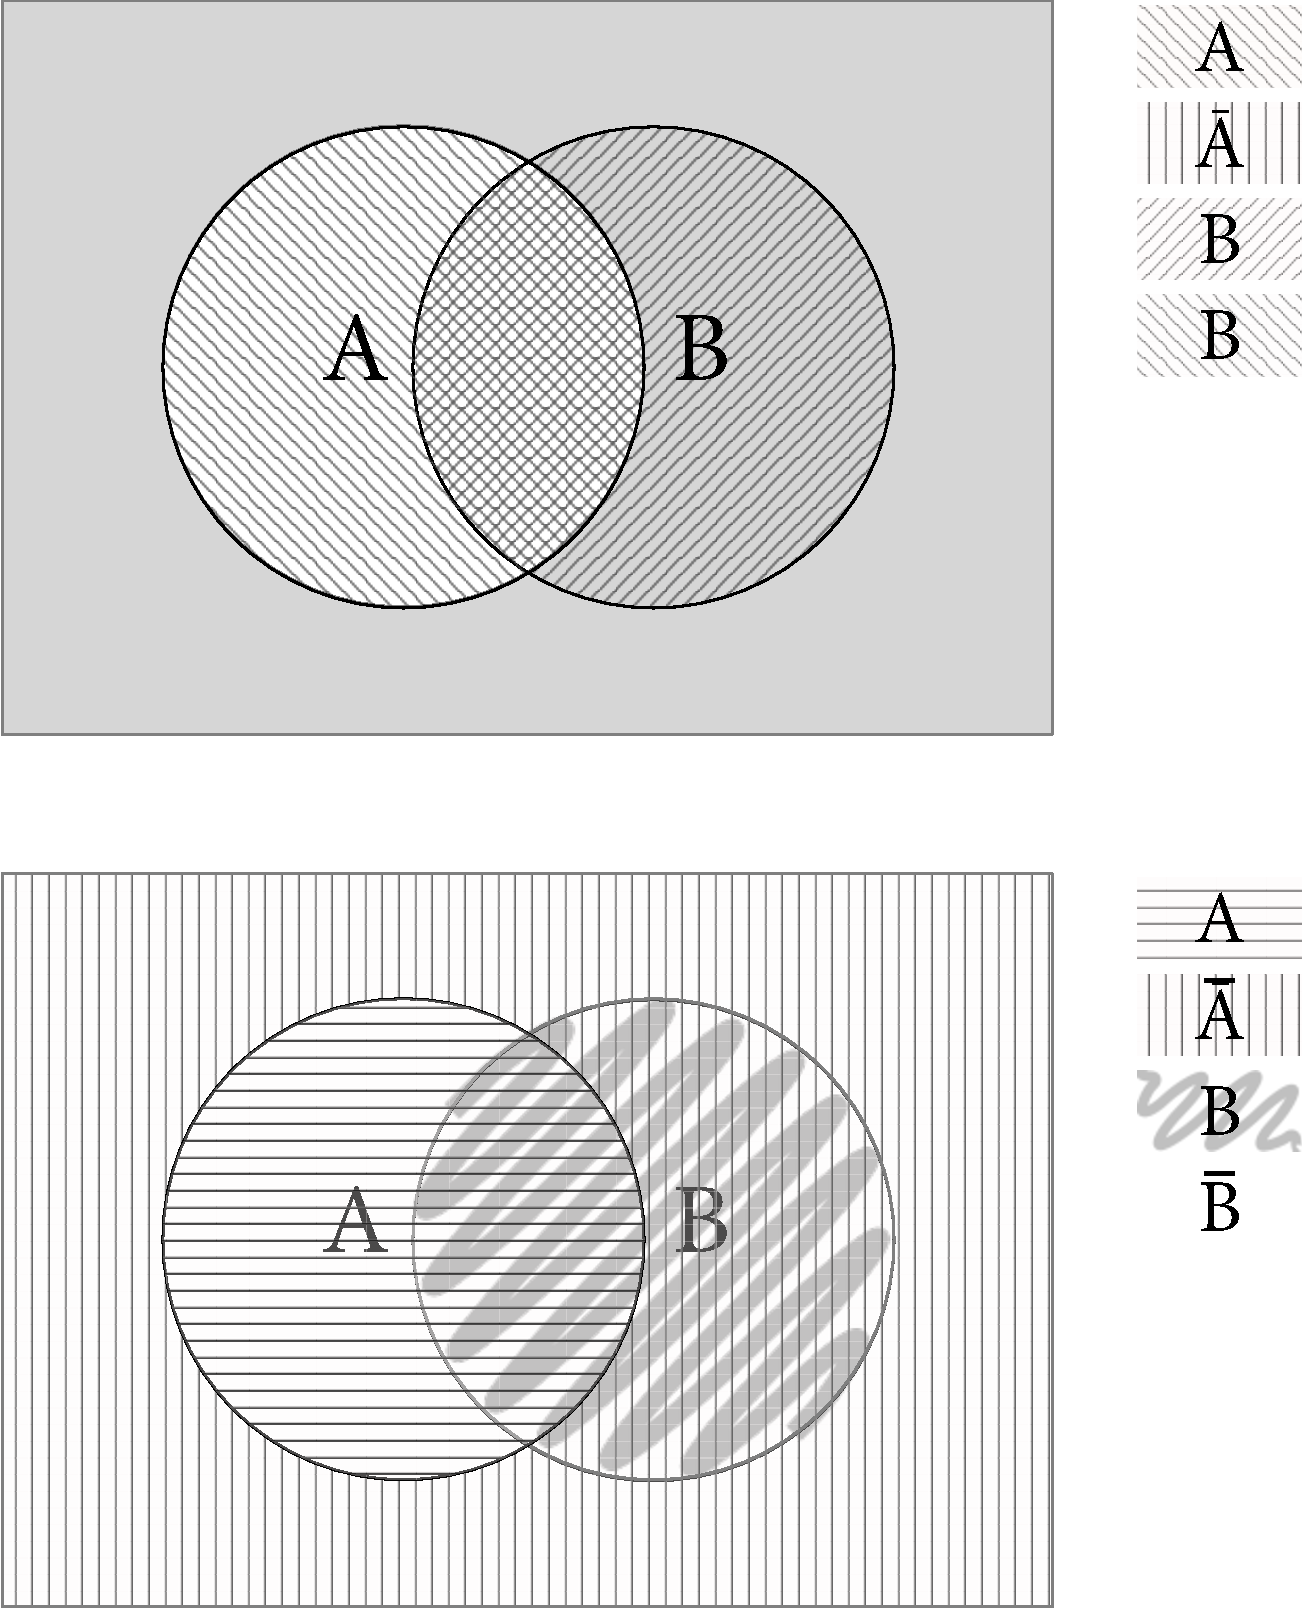
\includegraphics[width=6cm]{pic/VennDeMorganLaws.pdf}
\anngraphics{6cm}{pic/VennDeMorganLaws.png}{De Morgan's Laws for Sets are
exemplified through the labelling and shading of a Venn Diagram consisting
of two circles which overlap, each representing set A and B respectively.}
\end{center}
\caption{De~Morgan's Laws for Sets}
\label{figdemorganset}
\end{figure}

\begin{thm}[De~Morgan's laws]
Let $U$ be a set (a universe) with $A,B\subset U$.
Then (Figure~\ref{figdemorganset}):\\
a) $(A\cup B)^\mycomplement=A^\mycomplement\cap B^\mycomplement$.\\
b) $(A\cap B)^\mycomplement=A^\mycomplement\cup B^\mycomplement$.
\end{thm}
\begin{proof}
Again, to show equality of sets, we need to show inclusion in two directions:
a) Let $x\in (A\cup B)^\mycomplement$. That means that $x\in U$ but $x\not\in
A\cup B$. But that means that $x$ can be neither in $A$, nor in $B$, so
$x\in A^\mycomplement$ and $x\in B^\mycomplement$ and thus $x\in
A^\mycomplement\cap B^\mycomplement$.
Conversely, let $x\in A^\mycomplement\cap B^\mycomplement$.
That means that $x\in U$ but $x\not\in A$ and
$x\not\in B$, and thus $x\not\in A\cup B$. This implies that
$x\in(A\cup B)^\mycomplement$.\\
b) Exercise
\end{proof}

\subsection{Disjunctive Normal Form}

Using the laws introduced in the previous two sections, it is possible to
simplify a complicated expression involving sets into a simpler form. In
particular, it is possible to transform any such expression into a
\begin{itemize}
\itemsep-2mm
\item[] Union of
\begin{itemize}
\itemsep-2mm
\item[] Intersections of
\begin{itemize}
\itemsep-2mm
\item[] Sets or Complements of sets.
\end{itemize}
\end{itemize}
\end{itemize}
Such a form is called \defini{disjunctive normal form} (\defini{DNF}). For example,
\[
(A\cap B^\mycomplement\cap C)\cup (A^\mycomplement\cap D)
\]
is in DNF, while
\[
(A\cup B^\mycomplement\cup C)\cap (A^\mycomplement\cap D)^\mycomplement
\]
is not. However we can transform this expression stepwise into DNF:
\begin{eqnarray*}
&&(A\cup B^\mycomplement\cup C)\cap (A^\mycomplement\cap D)^\mycomplement\\
&=&(A\cup B^\mycomplement\cup C)\cap ((A^\mycomplement)^\mycomplement\cup
D^\mycomplement)\\
&=&(A\cup B^\mycomplement\cup C)\cap (A\cup D^\mycomplement)\\
&=&(A\cap (A\cup D^\mycomplement))\cup (B^\mycomplement\cap (A\cup
D^\mycomplement))\cup (C\cap (A\cup D^\mycomplement))\\
&=&(A\cap A)\cup (A\cap D^\mycomplement)\cup (B^\mycomplement\cap A)\cup
(B^\mycomplement\cap D^\mycomplement)\cup (C\cap A)\cup (C\cap D^\mycomplement)\\
&=&(A)\cup (A\cap D^\mycomplement)\cup (B^\mycomplement\cap A)\cup
(B^\mycomplement\cap D^\mycomplement)\cup (C\cap A)\cup (C\cap D^\mycomplement)\\
\end{eqnarray*}

If we imagine a Venn diagram of the sets, the disjunctive normal form
describes how the set can be composed from minimal intersecting parts.

\section{Connections to Logic}
\label{seclogic}

The distributive laws and De Morgan laws might to some readers look very
similar to statements about operations in logic. Here we have truth values
that can be true or false, and we can combine them with {\em and} (symbol
$\wedge$),
{\em or} (symbol $\vee$
\mynote{This is actually the origin of these symbols. The Latin
word for ``or'' is ``vel''.}),
and negate them (symbol $\lnot$). If we take distributive laws or De Morgan
laws and replace $\cap$ by $\wedge$, $\cup$ by $\vee$ and $\mycomplement$ by
$\lnot$ (placed before instead of exponents), we get the following valid
logic laws (we call the variables $P$, $Q$, and $R$ here):
\begin{enumerate}
\item $P\wedge (Q\vee R)=(P\wedge Q)\vee(P\wedge R)$.
\item $P\vee (Q\wedge R)=(P\vee Q)\wedge(P\vee R)$.
\item $\lnot(P\vee Q)=(\lnot P)\wedge (\lnot Q)$.
\item $\lnot(P\wedge Q)=(\lnot P)\vee (\lnot Q)$.
\end{enumerate}
The reason for this is easy, if we consider $P,Q,R$ as predicates (that is
functions that give truth values) for
objects in a set $U$ that are true for some elements and false for others.
We then define:
\begin{eqnarray*}
A&=&\{x\in U\mid P(x)=\mbox{true}\},\\
B&=&\{x\in U\mid Q(x)=\mbox{true}\},\\
C&=&\{x\in U\mid R(x)=\mbox{true}\},
\end{eqnarray*}
and observe that $A\cap B$ is the set of objects for which $P\wedge Q$ is
true, $A\cup B$ the set for which $P\vee Q$ is true and $A^\mycomplement$ the
set for which $\lnot P$ is true.
\medskip

In the same way as with sets we have a disjunctive normal form. That is
every logical expression can be written as an ``or'' combination of ``and''
combinations of variables or their negations.
Such a form can be useful in evaluating the truth value of a more
complicated logical expression, and there is a method (called the
{\em Quine-McCluskey algorithm}) to convert a logical expression into a
unique, minimal disjunctive normal form.

%rest of section by MM
We illustrate De~Morgan's laws and the distributive laws
(Section~\ref{demorganlaws})
with an example.
Let $U = \{ x \in \mathbb{Z} \mid 0 \leq x \leq 9 \} = \{0,1, \dots, 9\}$.
For this example, we will take complements of subsets of $U$.
Let
\[A = \{ x \in U \mid 0 \leq x \leq 4 \} = \{ 0, 1, 2, 3, 4 \}\]
\[B = \{ x \in U \mid x \text{ is even}\} = \{0,2,4,6,8\}.\]
For visualization, we can imagine the numbers in $A$ are colored red and the numbers in $B$ are written larger:
\[
\big\{\,
\textcolor{red}{\Large \textbf{0}},\textcolor{red}{1},\textcolor{red}{\Large\textbf{2}},\textcolor{red}{3},\textcolor{red}{\Large\textbf{4}},5,\textbf{\Large6},7,\textbf{\Large8},9
\,\big\}.
\]
We can use the first of De~Morgan's laws to find
\[
(A \cup B)^\mycomplement = A^\mycomplement \cap B^\mycomplement = \{ 5,6,7,8,9 \} \cap \{ 1,3,5,7,9 \} = \{ 5,7,9 \}.
\]
Viewing this in terms of operations in logic, we can interpret $A^\mycomplement \cap B^\mycomplement$ as the set of numbers in $U$ that are not red and not large.
This is in fact the complement of $A \cup B = \{ 0,1,2,3,4,6,8 \}$, which is the set of numbers in $U$ that are red or large (or both).
De~Morgan's law is simply an observation that such statements are two different ways to identify the same set.

Similarly, by applying the second of De~Morgan's laws, we find
\[
(A \cap B)^\mycomplement = A^\mycomplement \cup B^\mycomplement = \{ 5,6,7,8,9 \} \cup \{ 1,3,5,7,9 \} = \{ 1,3,5,6,7,8,9 \},
\]
and this is in fact the complement of $A \cap B = \{ 0,2,4 \}$.
We may interpret this second law as saying that the set of numbers in $U$ that are not both red and large is the same as the set of numbers that are not red or not large.

For an example of the distributive laws, let $C = A^\mycomplement = \{ 5,6,7,8,9 \}$; these are the numbers in $U$ that are not red.
Then
\[
A \cap (B \cup C) = \{ 0,1,2,3,4 \} \cap \{ 0,2,4,5,6,7,8,9 \} = \{ 0,2,4 \}
\]
and
\[
(A \cap B)\cup(A \cap C) = \{ 0,2,4 \} \cup \varnothing = \{ 0,2,4 \},
\]
so the distributive law $A \cap (B \cup C) = (A \cap B)\cup(A \cap C)$ holds.
Again, we may reinterpret this law as a logical statement, and each piece of the equations above can be described in these terms.
For instance, $A \cap C$ is the set of numbers in $U$ that are both red and not red, and therefore this is the empty set.


Likewise, we can verify that the other distributive law holds as well, since
\[
A \cup (B \cap C) = \{ 0,1,2,3,4 \} \cup \{ 6,8 \} = \{ 0,1,2,3,4,6,8 \}
\]
and
\[
(A \cup B)\cap(A \cup C) = \{0,1,2,3,4,6,8\} \cap U = \{0,1,2,3,4,6,8\},
\]
and thus $A \cup (B \cap C) = (A \cup B)\cap(A \cup C)$.



\section{Predicate Logic and Quantifiers}

Using predicates, we can start to construct mathematical statements. Such
statements typically assume that if some properties hold for an object (that
is some predicate $P$ has true value $P(x)$ on an element $x$), then some
other property holds (i.e. some other predicate $Q$ will have value $Q(x)$
as true. We can write this a $P(x)\Rightarrow Q(x)$, and combine predicates
with logical operations.

To write mathematical theorems, we however need two more operations, called
\defini{quantifiers}. They specify whether a predicate holds for all objects
in a set (e.g. {\em all cats are grey}), or if there is (at least) one
object for which the property holds (e.g. {\em there is a highest
mountain}). The former is called a \defini{universal statement}, the latter
an \defini{existence statement}.
We write down a universal statement
by writing down ``for all'' (often using the symbol $\forall$), followed by
naming an element from a set for which the property is to be stated. This
element stands for any (or all) elements of the set.
In the case of an existence statement we write ``there exists'' (using the
symbol $\exists$), again followed by selecting one element of a set, which
is to be the one element for which the following property is claimed.
For example,
using $E\subset\Z_{\ge 0}$ for the set of nonnegative even numbers, and
$D=\Z_{\ge 0}\setminus E$ for the
set of nonnegative odd numbers:
\begin{itemize}
\item The sum of an even number and $1$ is odd:
$\forall x\in E: x+1\in D$.
\item The sum of two odd numbers is even
$\forall x,y\in D:x+y\in E$
\item
The number $1234567$ is composite: $\exists x,y\in\Z; x,y>1: 1234567=x\cdot
y$.
\item
Every even number is a multiple of $2$: $\forall x\in E\exists y\in\Z:
x=2y$. (The $:$ here can be read as ``such that'').
\item
Every even number is (strictly) smaller than another even number:
$\forall x\in E\exists y\in E:y>x$.
\end{itemize}

Note that the order, in which we write the quantifiers of different type is important, and
that changing the ordering will change the meaning of the statement: For
example $\forall x\in\Z\exists y\in \Z: y=x+1$ ({\em for every integer there
exists one that is larger by one}, clearly a true statement) versus $\exists
y\in \Z\forall x\in\Z: y=x+1$ ({\em there is an integer ($y$) that is one
larger than every other integer}, a nonsensical claim).
(Adjacent quantifiers of the same type can be exchanged.)
\medskip

Most mathematical statements (either as part of a definition, or in the
claim of a theorem) can be formulated as a combination of $\exists$,
$\forall$, $:$, and $\Rightarrow$ (implication) statements. A formal proof
of such a statement then will follow this pattern:
\begin{center}
\begin{tabular}{c|c}
If the statement starts with:&Then the proof:\\
\hline
\begin{minipage}[t]{4cm}
An existence statement: $\exists x\in S\ldots$
\end{minipage}&\begin{minipage}[t]{6cm}
Construct (or describe a way how to find; effectively it will be an
algorithm) an element $x\in S$ that has
the required property (which will be given in the following part of the
statement).\\
A rarer, more complicated, construction is to imply
that such an element must exist, without giving an explicit way of finding
it. Such a proof would be called \defini{non-constructive}, and not allow
translation to an effective algorithm.
\end{minipage}\\
\hline
\begin{minipage}[t]{4cm}
A universal statement: $\forall x\in S\ldots$.
\end{minipage}&\begin{minipage}[t]{6cm}
The proof will start with a sentence: ``Let $x\in S$'' (and the implicit
fact that $x$ is to be an arbitrary element, or that any element of $S$
could be selected here). Then the proof will need to show that the remaining
part of the statement holds for $x$. For this we can use only the fact that
$x\in S$ (and the properties implied by it).
\end{minipage}\\
\hline
\begin{minipage}[t]{4cm}
An implication between predicates $P(x)\Rightarrow Q(x)$.
\end{minipage}&\begin{minipage}[t]{6cm}
We assume that the element $x$ satisfies the predicate $P$, and need to
shows that $x$ also satisfies the predicate $Q$.
\end{minipage}\\
\end{tabular}
\end{center}

\section{Pairs, Tuples, Cartesian Product}

In general, we do not store all items we use in big bags that get everything
thrown in together. Instead we often use more structured storage, say boxes
in drawers.
The same is true in mathematics,
where we will often find it convenient to have objects stored in a form with
more structure than a set. This section describes some of the ways how this
can be done.

We start with the definition of pairs: A \defini{pair} is an object $(a,b)$,
that holds two objects (namely $a$ and $b$) in two distinct positions,
enclosed by parentheses (or sometimes brackets: $[a,b]$). The
pair $(1,2)$ is different from the pair $(2,1)$, while the sets $\{1,2\}$
and $\{2,1\}$ are the same. (Note that sets and tuples formally are
different: $\{1,2\}\not=(1,2)$.)

Formally, we can construct pairs as sets. We simply define $(a,b)$ as a
shorthand for the set $\{a,\{a,b\}\}$. Note that this form allows us to
always extract the first ($a$) and second ($b$) entry unambiguously. (The
reason for building pairs from sets is that it allows to re-use existing
language and theorems, rather than having to re-do everything for the new
kind of objects.)
\medskip

If we have two sets $A,B$, we sometimes want to look at the set of all
possible pairs whose first entry is from $A$ and whose second entry is from
$b$.
This set is called the \defini{Cartesian product}\mynote{Named after the French
mathematician \person{Ren\'e Descartes}, who invented the standard $x/y$ coordinate set,
the \defini{Cartesian coordinates}, in which points are described by pairs.}
of $A$ with
$B$ and written as
\[
A\times B=\{(a,b)\mid a\in A,b\in B\}
\]
For example, if $A=\{1,2,3\}$ and $B=\{5,6\}$, then
\[
A\times B=\{(1,5),(1,6),(2,5),(2,6),(3,5),(3,6)\}
\]

It is easy to see that if $\sz{A}=m$ and $\sz{B}=n$, then $\sz{A\times
B}=m\cdot n$.
\medskip

The same process that leads to pairs can be extended or repeated (e.g by
forming pairs, whose entries are pairs again) and thus form ordered
collections of more than two objects, such as $(a,b,c)$ or $(3,1,4,1,5,9)$.
We call such objects \defini{tuples},
typically together with a number that
indicates the number of entries.
Thus $(7,3,5)$ is a $3$-tuple and $(8,2,5,1,4,1,2)$ an $7$-tuple; pairs
could be called $2$-tuples.
And of course the set of all $k$-tuples can be considered as an iterated
Cartesian product $A\times B\times C\times\cdots\times K$.
\medskip

Conceptually, pairs and tuples will allow us to group information consisting
of different parts (that may not be mixed up) together. It is the first step
towards structured data.

\subsection{Indexing and index sets}

If we have a tuple, we might want to refer to a
particular entry of it. The easiest way to do so is by referring to the
place in the tuple, at which the entry lies. We often do so by adding an
\defini{index} to the name of the tuple,
that is a number put on the bottom right of the object. For
example, if $t=(p,r,q)$, we have $t_1=p$, $t_2=r$ and $t_3=q$. (Sometimes
people like to start at $0$ instead. Which convention is used needs to be
stated or be clear from the context.) We thus could write
\[
t=(t_1,t_2,\ldots,t_k)
\]
for a particular $k$-tuple. Programmers might prefer to write $t[i]$ instead. The
index notation simply uses less ink and space.
\smallskip

We can put the possible positions (i.e. the possible indices) into an
\defini{index set}, and use this to refer to the entries: Let
$I=\{1,2,\ldots,k\}$ and we will talk about $t_i$
for $i\in I$.  \mynote{The reader who already has some programming
experience should think at this point of a \texttt{for}-loop. The $i$ (for
``index'') from mathematics is also the reason that the standard name of a
loop variable is \texttt{i} as well.}
\smallskip

This concept (and notation) generalizes easily to other, even infinite, index
sets. We might take an index set $P$ of persons and then talk of the first
name $f_p$ for a person $p\in P$. Or we look at entries $t_i$, $i\in\N$ for
an infinite tuple (which we will call a sequence~\pointer{secsequences})
$(t_1,t_2,t_3,\ldots)$.

Mathematics here only cares about the fact that the indexed object $t_i$ is
determined clearly and unambiguously from the index $i$, while implementing
such objects on a computer, in particular for more complicated index sets,
can bring up questions of efficiency -- finding the object associated to a
particular index.  But that is a topic you will learn about in courses on
algorithms and data structures.
\medskip

The entries of a tuple can be tuples again, and we can refer to the entries
of entries by multiple indices. Here one typically will write $t_{i,j}$
instead of a more clumsy $(t_i)_j$.
For example, suppose we have a $2$-tuple $t$
(depicted here written vertically), whose entries are $3$-tuples. We then
can refer to the entries of this object (also called a~\defini{matrix}) as
follows
\[
\begin{array}{rcl}
\left(\quad(t_{1,1},\right.&t_{1,2},&t_{1,3}),\\
(t_{2,1},&t_{2,2},&t_{2,3})\left.\quad\right).\\
\end{array}
\]
Contrary to the $x/y$ coordinates of geometry, here the first entry
typically indexes the row and the second entry the column. Again this can
be generalized to objects of higher dimension

\subsection{Generating Tuples and Subsets}

%KB, edited AH

In understanding tuples and index sets, it can be helpful to think about how
one would generate such objects in algorithms. First, lets look how an
algorithm would generate all pairs in $A\times B$: We select all
possibilities for the first entry and for each such choice select all
possibilities for the second entry. If the sets $A$ and $B$
are given as input, this is simply a set of iterated \texttt{for} loops:
\begin{verbatim}
for a in A do
  for b in B do
    print (a,b); # or other processing, as desired
  od;
od;
\end{verbatim}
If we replaced the second \texttt{for} loop by \texttt{for b in A do}, we
would get the pairs in $A\times A$. To enumerate $A\times A\times A$ would be
three iterated for loops and so on.
\medskip

To describe all subsets of a set, we re-use the idea we already
encountered in Section~\ref{secpowerset}, of indicating by bits whether an
element lies in the set or not. If we have a set $A$ with $n$ elements, the
subsets thus can be described as $n$-tuples in
$\underbrace{B\times\cdots\times B}_{\mbox{$n$ factors}}$ where $B=\{0,1\}$.
For example, if $n=3$, the following algorithm would construct these subsets
\begin{verbatim}
for a in {0,1} do
  for b in {0,1} do
    for c in {0,1} do
      print (a,b,c);
    od;
  od;
od;
\end{verbatim}
(Writing such an algorithm for an {\em arbitrary} (user-selected) value of
$n$ is a bit more difficult, and recursion might be the easiest way to do
so.)

In using bit lists to describe subsets we of course need to fix an ordering
of the elements of $A$. For example if we have
$A=\{\text{dog},\text{bird},\text{cat}\}$, and consider the elements in this
order, we get the following correspondences:
\begin{align*}
(0,0,0) &\longleftrightarrow \emptyset\\
(1,0,1) &\longleftrightarrow \{\text{dog},\text{cat}\}\\
(0,1,0) &\longleftrightarrow \{\text{bird}\}\\
(1,1,1) &\longleftrightarrow \{\text{dog},\text{bird},\text{cat}\}.
\end{align*}
But if we used
$A=\{\text{dog},\text{cat},\text{bird}\}$ (this is the {\em same} set, we
just change the convention in how we order elements), the tuple $(1,0,1)$ would
describe the subset $A=\{\text{dog},\text{bird}\}$. (Formally, each
arrangement give us a different
bijective function between the binary tuples and the subsets.)

\subsection{Multisets}
\label{secmultiset}

We can use the construct of an index set to associate counts to objects of a
set and thus represent objects being in a set multiple times. The resulting
object is called a \defini{multiset}. Formally, a multiset can be defined as
an ordinary set $S$, together with a counting set $C=\{c_s\in\N\mid s\in
S\}$ indexed by $S$. This pair $(S,C)$ then represents a collection in which
object $s\in S$ occurs  $c_s$ times. For example, we could describe a
wallet's content by the set $S=\{p,n,d,q\}$ \mynote{US-centric {\em
penny} (1 cent) ,{\em nickel} (5 cent),{\em dime} (10 cent), {\em quarter} (25 cent).}
and have e.g.
\[
W=(S,C),\quad C=\{c_p=3,c_n=1,c_d=0,c_q=3\}.
\]
